The locus of the Orthocenter $X_4$ is an ellipse of axes $a_4,b_4$ similar to a rotated copy of the EB. These are given by \cite {garcia2020-ellipses}:
%
\begin{equation*}
\left(a_4,b_4\right)=\left(\frac{k_4}{a},\frac{k_4}{b}\right),\;  k_4=\frac{  ({a}^{2}+{b}^{2})\delta-2\,{a}^{2}{b}^{2} }{c^2}    
\end{equation*}
%
\noindent Referring to Figure~\ref{fig:orthocenter_loci}, let $\alpha_4=\sqrt{2\,\sqrt {2}-1}\;{\simeq}\;1.352$.

\begin{proposition}
If $a/b=\alpha_4$, then $b_4=b$, i.e., the top and bottom vertices of the locus of $X_4$ coincide with the EB's top and bottom vertices.
\end{proposition}

\begin{proof}
The equation $b_4=b$ is equivalent to $a^4+2a^2b^2-7b^4=0.$ Therefore, as $a>b>0$, it follows that $a/b=\sqrt{2\,\sqrt {2}-1}.$
\end{proof}

\noindent Let $\alpha_4^*$ be the positive root of
${x}^{6}+{x}^{4}-4\,{x}^{3}-{x}^{2}-1=0$, i.e.,
$\alpha_4^{*}={\simeq}\;1.51$. 

\begin{proposition}
When $a/b=\alpha_4^{*}$, then $a_4=b$ and $b_4=a$, i.e., the locus of $X_4$ is identical to a rotated copy of Billiard. 
\end{proposition}

\begin{proof}
The condition $a_4=b$, or equivalently $b_4=a$, is defined by $a^6+a^4b^2-4a^3b^3-a^2b^4-b^6=0$. Graphic analysis shows that ${x}^{6}+{x}^{4}-4\,{x}^{3}-{x}^{2}-1=0$ has only one positive real root which we call $\alpha_4^*$.
\end{proof}

\begin{theorem}
If $a/b<\alpha_4$ (resp. $a/b>\alpha_4$) the 3-periodic family will not (resp. will) contain obtuse triangles.
\end{theorem}

\begin{proof}
If the 3-periodic is acute, $X_4$ is in its interior, therefore also internal to the EB. If the 3-periodic is a right triangle, $X_4$ lies on the right-angle vertex and is therefore on the EB. If the 3-periodic is obtuse, $X_4$ lies on exterior wedge between sides incident on the obtuse vertex (feet of altitudes are exterior). Since the latter is on the EB, $X_4$ is exterior to the EB.
\end{proof}

\begin{figure}[H]
    \centering
    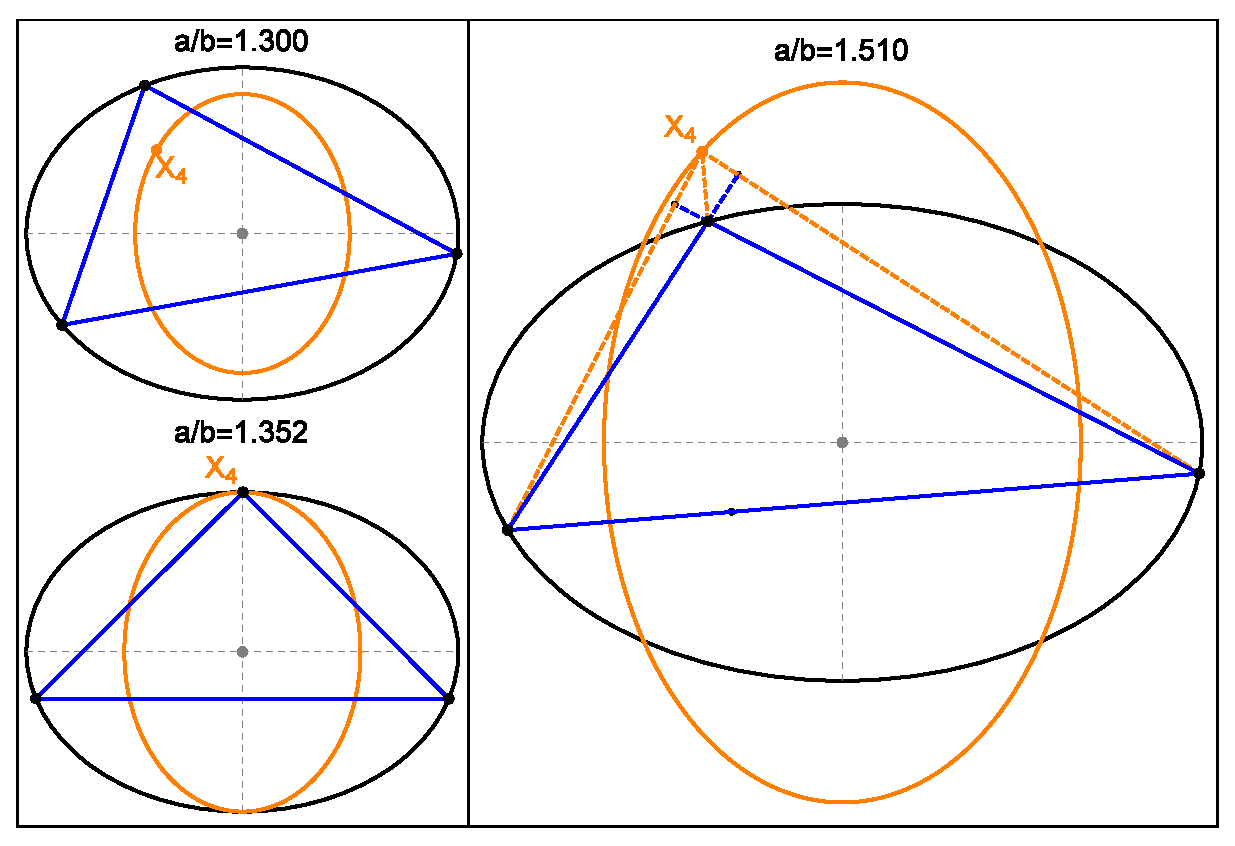
\includegraphics[width=.8\textwidth]{pics/1010_ort_loci.eps}
    \caption{Let
    $\alpha_4=\sqrt{2\,\sqrt {2}-1}\;{\simeq}\;1.352$
    and $H$ be the elliptic locus of $X_4$ (orange), similar to a rotated copy of the EB (black). \textbf{Top Left}: $a/b<\alpha_4$, $H$ is interior to the EB and all 3-periodics (blue) are acute. \textbf{Bot Left}: at $a/b=\alpha_4$, $H$ is tangent to the top and bottom vertices of the EB. The 3-periodic shown is a right triangle since one vertex is at the upper EB vertex where $X_4$ currently is. \textbf{Right}: at $a/b>\alpha_4$, the 3-periodic family will contain both acute and obtuse 3-periodics, corresponding to $X_4$ interior (resp. exterior) to the EB. For any obtuse 3-periodic, $X_4$ will lie within the wedge between sides incident upon the obtuse angle and exterior to the 3-periodic, i.e., exterior to the EB. For the particular aspect ratio shown ($a/b=1.51$), $H$ is identical to a $90^{\circ}$-rotated copy of the EB.}
    \label{fig:orthocenter_loci}
\end{figure}

